\section{Transformation of the equations}\label{sec:transformationequations}

Having established the definition of the sum of normal distributions in \cref{sec:third_normal} to enhance mathematical tractability, we now delve into the transformation of equations from the existing binormal representation used in CLUBB-SILHS\cite{larson2022clubbsilhs} to a trinormal one.
While the formulas for the binormal case are well-defined, the simplicity of the means and standard deviations employed in the trinormal representation suggests the existence of a specific transformation that holds true.
This chapter will demonstrate that the following transformations, denoted by the subscript \enquote{dGn} for the binormal case, successfully achieve this conversion.

\begin{align}
    \overline{w'^2} \frac{1 - \delta\lambda_w}{1 - \delta}
    &= \overline{w'^2}_{dGn}, \label{eq:w_prime_2_transform}
\end{align}
\begin{align}
    \overline{w'^3} \frac{1}{1 - \delta}
    &= \overline{w'^3}_{dGn}, \label{eq:w_prime_3_transform}
\end{align}
\begin{align}
    \frac{\overline{w'^3}}{\overline{w'^2}^{3/2}} \frac{(1 - \delta)^{1/2}}{(1 - \lambda_w\delta)^{3/2}}
    &= \frac{\overline{w'^3}_{dGn}}{\overline{w'^2}_{dGn}^{3/2}}, \label{eq:w_prime_3_div_w_prime_2_transform}
\end{align}
\begin{align}
    \overline{\theta_l'^2} \frac{1 - \delta\lambda_\theta}{1 - \delta}
    &= \overline{\theta_l'^2}_{dGn}, \label{eq:theta_l_prime_transform}
\end{align}
\begin{align}
    \overline{w'\theta_l'} \frac{1 - \delta\lambda_{w\theta}}{1 - \delta}
    &= \overline{w'\theta_l'}_{dGn}, \label{eq:w_prime_theta_l_prime_transform}
\end{align}
\begin{align}
    \left(\overline{w'^4} - 3\delta\lambda_w^2 \left(\overline{w'^2}\right)^2\right) \frac{1}{1 - \delta}
    &= \overline{w'^4}_{dGn} \label{eq:w_prime_4_transform}
\end{align}
\begin{align}
    \left(\frac{\overline{w'^4}}{(\overline{w'^2})^2} - 3\delta\lambda_w^2 \right) \frac{1 - \delta}{(1 - \lambda_w\delta)^2}
    &= \frac{\overline{w'^4}_{dGn}}{(\overline{w'^2}_{dGn})^2} \label{eq:w_prime_4_div_w_prime_2_transform}
\end{align}

To get a sense of what those transformations mean and why they should work, we pick e.g. \cref{eq:w_prime_2_transform}.
If we substitute in the already defined formula for $\lambda_w$ (\cref{eq:lambda}), we get
\begin{align*}
    \overline{w'^2} \frac{1 - \delta\lambda_w}{1 - \delta}
    &= \overline{w'^2}_{dGn} \\
    \overline{w'^2} (1 - \delta\frac{\sigma_{w 3}}{\wptwo})
    &= (1 - \delta)\overline{w'^2}_{dGn} \\
    \overline{w'^2} - \delta\sigma_{w 3}
    &= (1 - \delta)\overline{w'^2}_{dGn} \\
    \overline{w'^2}
    &= \overline{w'^2}_{dGn} - \delta\overline{w'^2}_{dGn} + \delta\sigma_{w 3} \\
    \overline{w'^2}
    &= \overline{w'^2}_{dGn} - \delta\left(\overline{w'^2}_{dGn} - \sigma_{w 3}\right)
\end{align*}
which suggests that if we set $\delta=0$ that we revert back to the binormal case, exactly as wanted.
We see that the overall variance (\enquote{width}) of the sum depends on the standard deviation of the third normal more and more as $\delta$ approaches 1 (it can not exactly reach 1).

Also, if we look at \cref{eq:w_prime_3_transform}, we see that there is no more $\lambda_w$ present.
\begin{align*}
    \overline{w'^3} = (1 - \delta)\overline{w'^3}_{dGn}
\end{align*}
Looking at this formula, it makes sense graphically, that as delta grows, which means that the normal \gls{pdf} in the middle is growing, the overall skewness of all three normals has to change also, depending on the value of $\sigma_{w 3}$.
We can see this in \autoref{fig:1dplotbitri}, where we fix the following variables: $w_1 = 5$, $w_2 = -5$, $\alpha = 0.5$, $\sigma_w = 2$, and $\delta = 0.5$.

\begin{figure}
    \centering
    \begin{tabular}{cc}
        \multicolumn{1}{c}{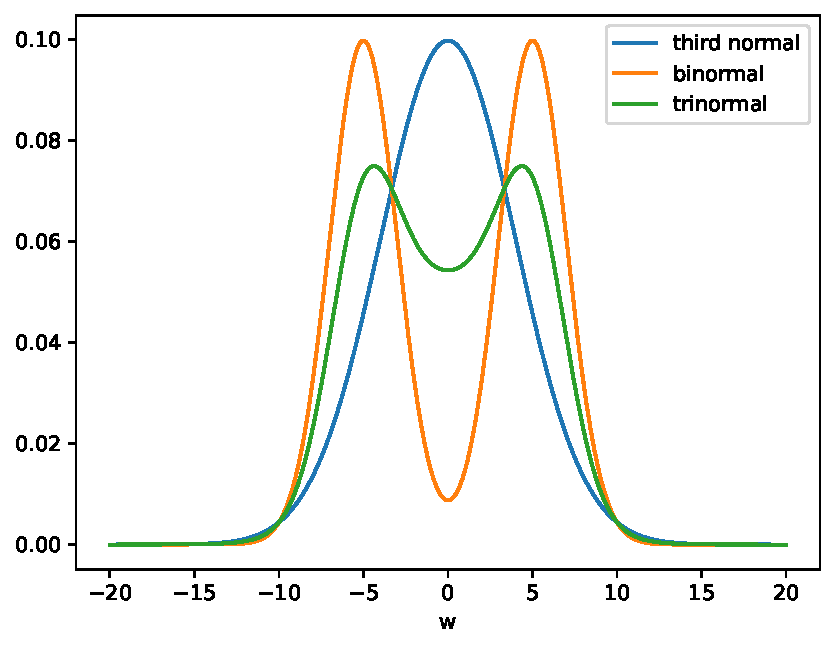
\includegraphics[width=0.48\textwidth]{include/figures/1dplotslw4}} &
        \multicolumn{1}{c}{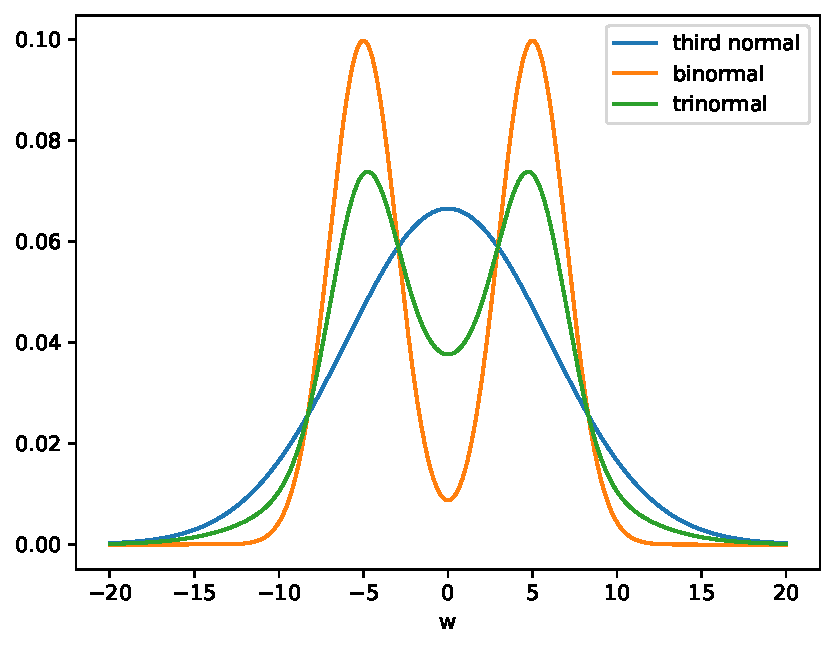
\includegraphics[width=0.48\textwidth]{include/figures/1dplotslw6}} \\
        $\sigma_{w3} = 4$ & $\sigma_{w3} = 6$  \\ \\
        \multicolumn{1}{c}{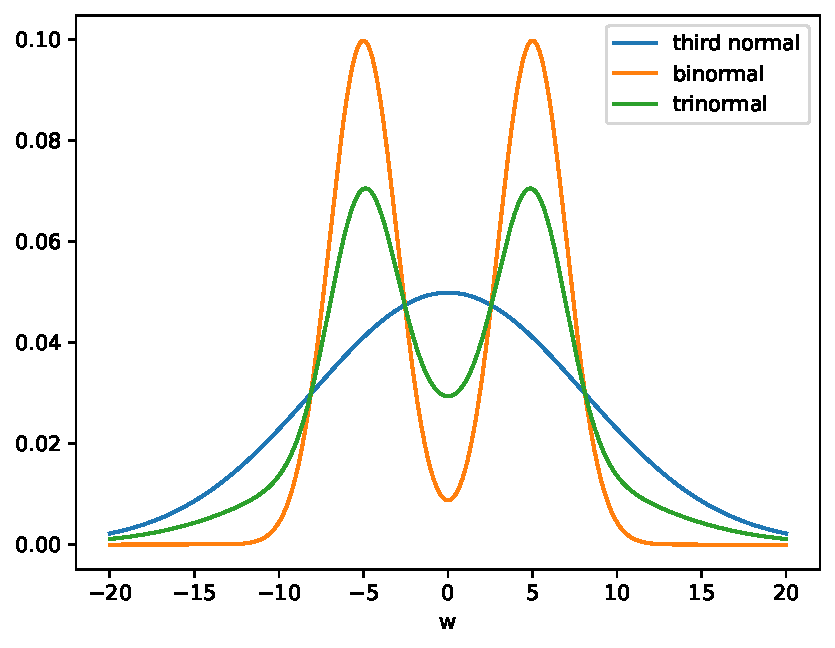
\includegraphics[width=0.48\textwidth]{include/figures/1dplotslw8}} &
        \multicolumn{1}{c}{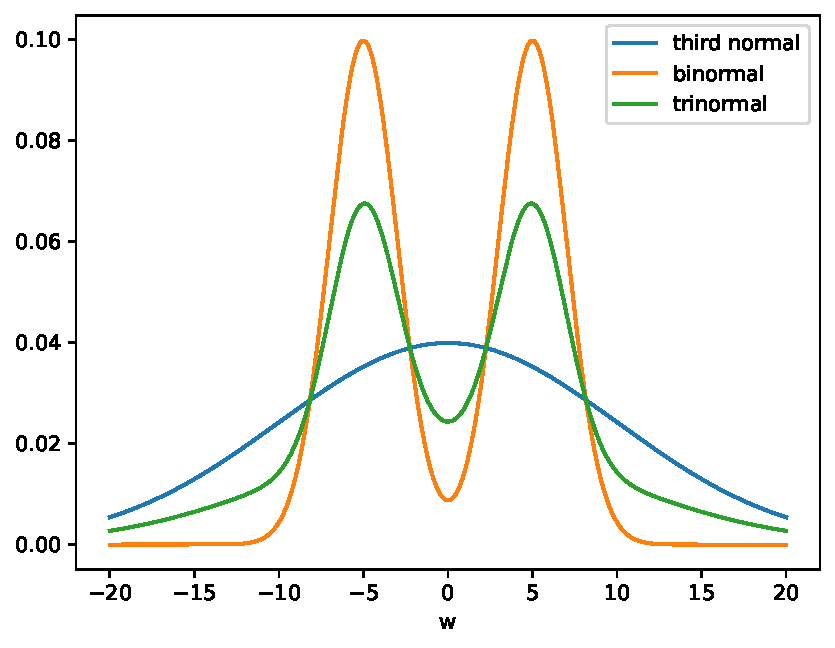
\includegraphics[width=0.48\textwidth]{include/figures/1dplotslw10}} \\
        $\sigma_{w3} = 8$ & $\sigma_{w3} = 10$
    \end{tabular}
    \caption{1D plot for binormal and trinormal case}
    \label{fig:1dplotbitri}
\end{figure}
